\chapter{Results}\label{chap:results}
\thispagestyle{fancy}

\section{Cataclysmic Variables }
From the population of known CV candidates in NGC 6397, we were able to get the spectra of five of them (see Figure~\ref{fig:todosspectra}). In addition to recovering 3 of the previously identified cataclysmic variables, we have obtained the spectra for the first time of two CV candidates (U10 and U22 see figures \ref{fig:U10spectra} and \ref{fig:U22spectra}).  Their spectra confirm that these star are CVs, as suggested by their X-ray data \citep{grindlay_chandra_2001}. All the extracted spectra show the most common spectral lines detected from CVs. The most noticeable feature present in all the spectra are the Balmer lines. These are a set of spectral line emissions of the hydrogen atom. In the MUSE spectral range the H$\alpha$ ($6562 \text{ \r A}$) and H$\beta$ (4861 $\text{ \r A}$) lines are detectable. These lines are known to show a double-peaked profile, characteristic of an accretion disc. The red and blue peaks are formed by the emission from the receding and approaching parts of the edge of an accretion disk. With the exception of U10, all the obtained spectra lie within a distance of $11"$ from the cluster center. Their spectra is obtained from two observing nights of the cluster center. The total exposure time is 340 seconds from a total of 8 different exposures ($4 \times 25$ s and $4 \times 60$ s). U10 lies at a distance of $1.21'$ and was also observed during two different nights. The total exposure time on U10 is 265 seconds divided in 9 short exposures ($5 \times 25$ s and $4 \times 35$ s).

\begin{figure}[]
        \centering
        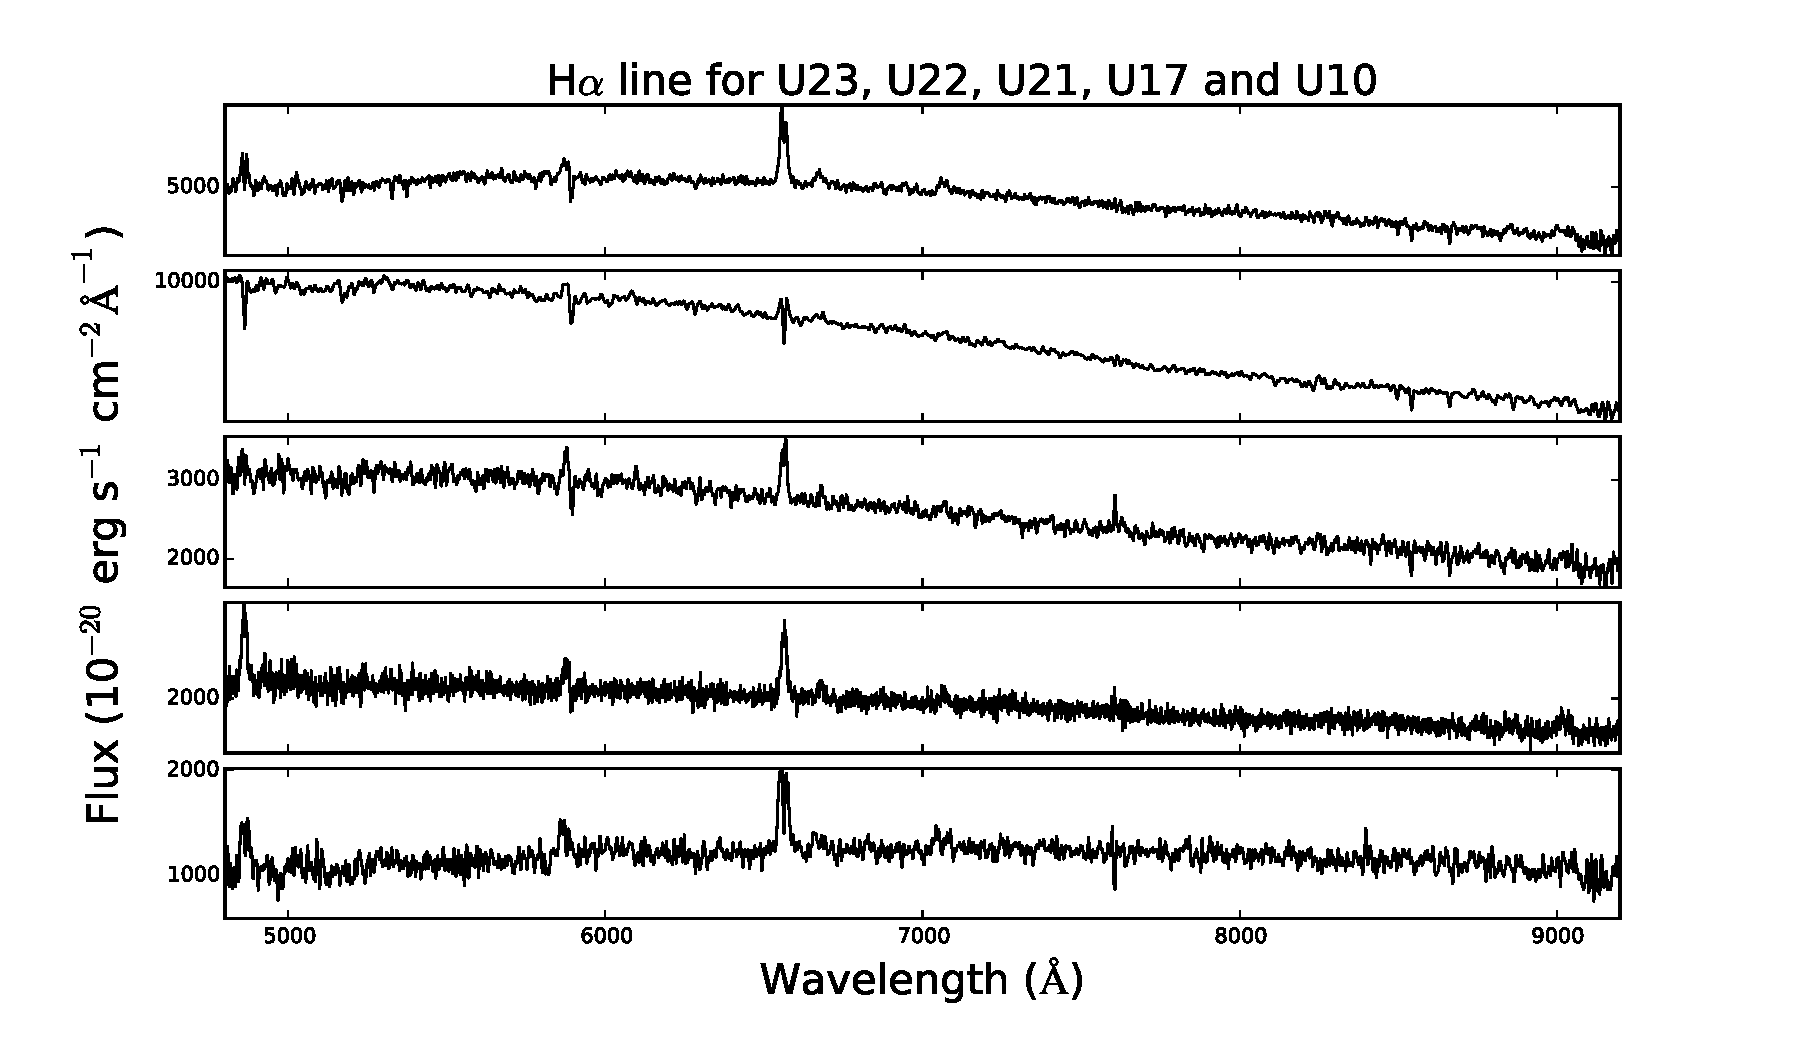
\includegraphics[scale=.6]{assets/images/todostodos.pdf}
\caption{Obtained spectra from CVs in NGC 6397. Three of them have been previously identified as CVs: U23, U21 and U17 \citep{grindlay_spectroscopic_1995,edmonds_cataclysmic_1999}. U22 and  U10 were CV candidates that we confirmed with spectroscopy for the first time. All CVs show strong Balmer lines ($ \text H \alpha \, 6563 \text{ and H}\beta \,  4861 \text{ \r A}$). The IDs are from \cite{bogdanov_chandra_2010}.}
\label{fig:todosspectra}
\end{figure}

\begin{figure}[]
        \centering
        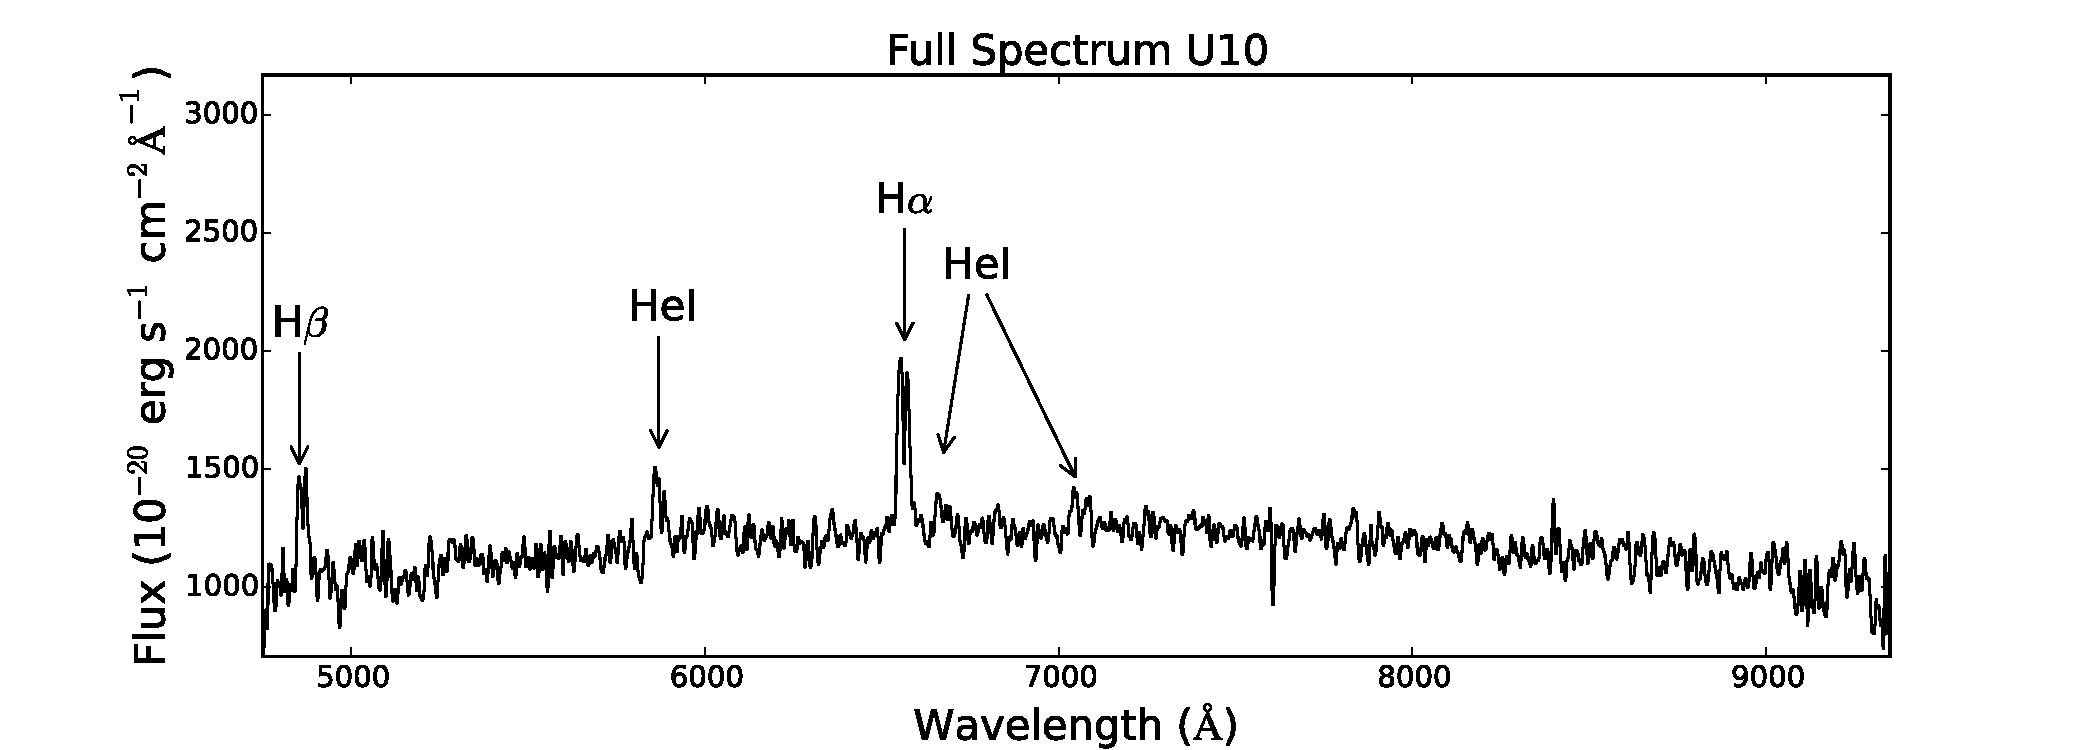
\includegraphics[scale=.5]{assets/images/U10full.pdf}
\caption{Spectrum of U23 with strong Hydrogen double peaked emission (characteristic of an accretion disk), and strong Helium I lines. }
\label{fig:U10spectra}
\end{figure}

\begin{figure}[]
        \centering
        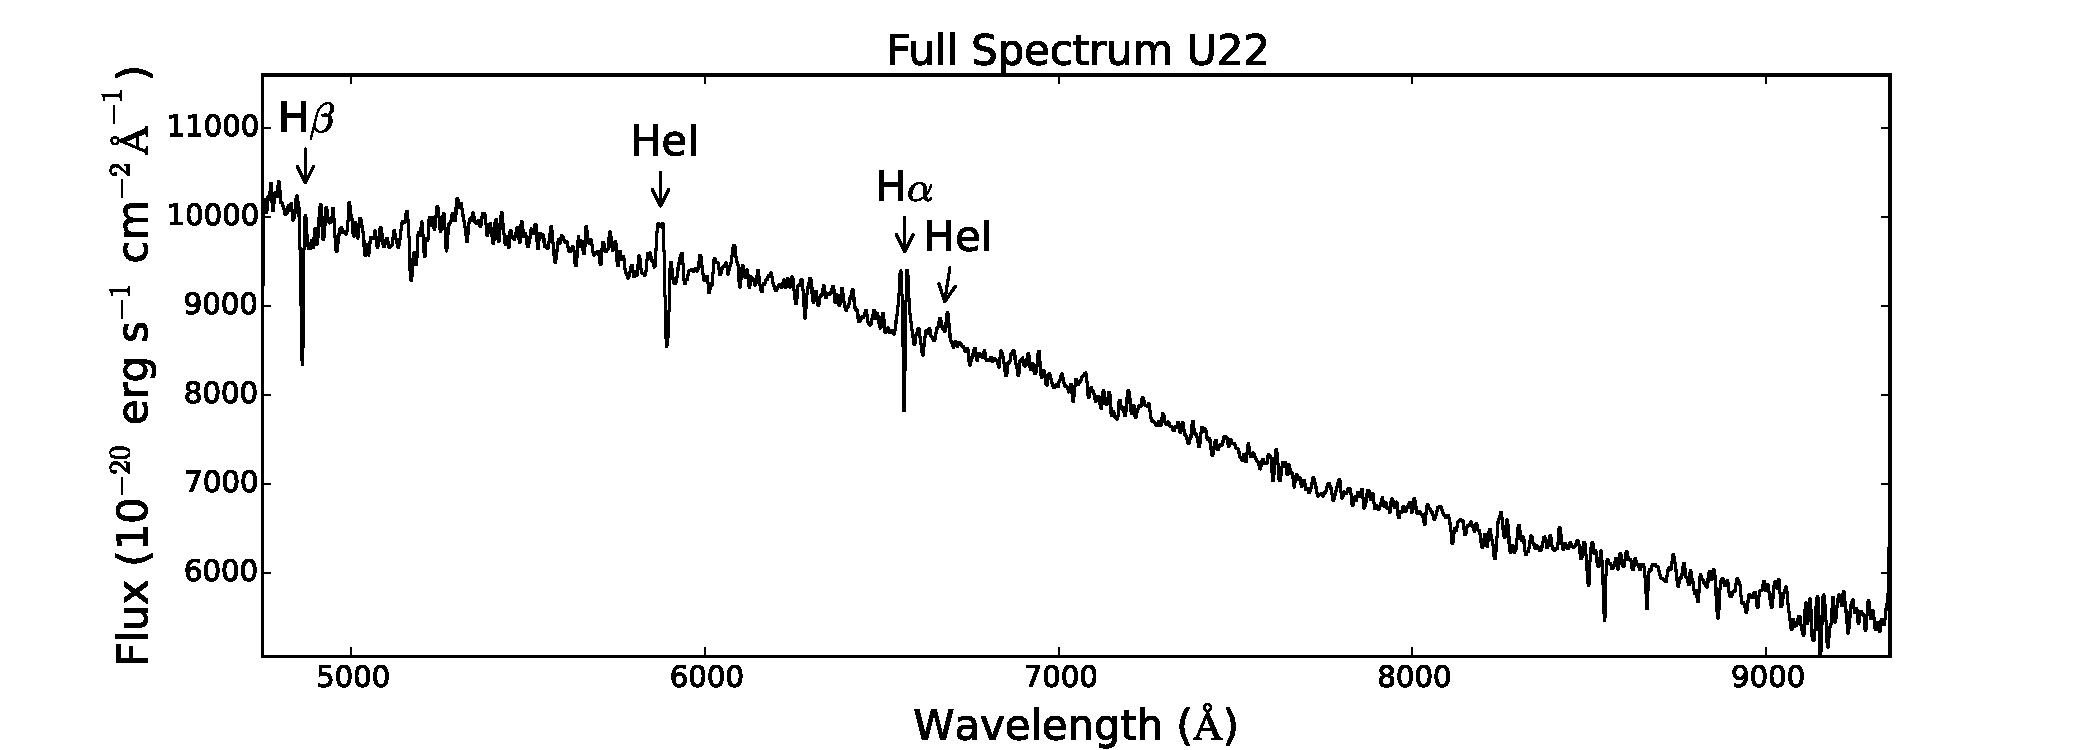
\includegraphics[scale=.5]{assets/images/U22full.pdf}
\caption{Spectrum of U22 with strong H$\alpha$ double peaked emission, absorption in the H$\beta$ line, and Helium I lines.}
\label{fig:U22spectra}
\end{figure}


\subsection{Variability}

From the extracted CV spectra, we calculated the magnitudes in the R band (in the VEGA system), and compare it to the magnitude seen in 2010 by the Hubble space telescope as reported by \cite{cohn_identification_2010}. The results are summarized in Table~\ref{tab:truthTables}. The CVs show moderate amplitude variability between the two observing times. This suggests that the majority of the CVs were observed during quiescence and not during an outburst. For some CVs like U22 where the change magnitude is bigger, but still also consistent with no variavirility, the possibility of being observed during outburst is not ruled out. A dwarf nova eruption can result in moderate magnitude changes of $\sim 2$. This has been observed for U17 and U19. They have been reported to undergo dwarf nova eruptions with amplitudes of 1.8 and 2.7 magnitudes \citep{shara_erupting_2005}. 




\begin{comment}
From shara both 96 and the discover yin NGC 6624
        The
probability of a typical field DN being in quiescence at any
given epoch is 0.85 (Szkody \& Mattei 1984). Thus the likelihood
of any DN being in quiescence during all three epochs
is just 10.853 1 0.6. We should thus have detected, on the
basis of eruptions alone, at least 40% of all DNs in the core
of NGC 6624. The total number of DNs in the core of
NGC 6624 cannot be much larger than the observed number/
detection efficiency (1/0.4 5 2.5).

From Sevillat and Webb
 The DN population constitutes about half of the
known CVs listed in the catalog of Downes et al. (2001), which
contain mostly field CVs. We could then expect ∼78 DNe in
M13, based on those rough estimations. The mean duty cycle,
or probability of a DN being in outburst at a random epoch, has
been found to be ∼15% based on the observation of 21 DNe
(Szkody & Mattei 1984). We can group our observations into
five epochs of few days, thus the likelihood of a DN being in
quiescence in those five epochs is 0.855 = 0.44. Thus, ∼42
DNe should have been in outburst in at least one of the epochs.
It is then harder to estimate the number of outbursts that would
have been bright enough to be detected in our observation. Our
detection limit at U ∼ 19 would convert to V ∼ 20 (MV ∼ 5.7)
due to the general blue color of DN outbursts (Harrison et al.
2004). We can then use the distribution of V magnitudes at maximum
light from Patterson (2011) based on the observations of
∼45 DNe, which shows that we could have expected to detect at
least two-third of those DNe in outburst at the distance of M13.
Finally, ∼28 DNe in outburst would have been expected when
we detect only one.

\end{comment}

%Further analysis of the spectra is needed to rule out the outburst scenario.  

\begin{table}[]
\centering
\begin{tabular}{|c|c|c|c|}
\hline
\textbf{CV} & \textbf{R Magnitude (2014)} & \textbf{R $\mathbf{\pm \, 0.002}$ (Cohn et al. 2010)} & \textbf{Variability}\\ \hline
U17         & $20.12 \pm 0.3$                       & 18.52  & Yes ($> 3 \sigma$)\\ \hline
U23         & $19.15 \pm 0.5$                      & 17.88  & Marginal $\sim 2.7 \sigma$                    \\ \hline
U10         & $20.7 \pm 1 $                        & 19.14 & No ($< 2 \sigma$)          \\ \hline
U21         & $19.79 \pm 0.3$                   & 19.82 & No \\ \hline
U22         & $18.54 \pm 0.9 $                       & 20.15 & No ($< 2 \sigma$)                              \\ \hline

\end{tabular}
   \caption{Magnitudes in the R band for the 5 CVs detected by MUSE in 2014 and the R magnitudes in 2010 studied by \cite{cohn_identification_2010}. Some CVs show small magnitude variability between the two epochs ($\sim 1$ magnitude).}
    \label{tab:truthTables}   
\end{table}





\begin{comment}
Results:

    Spectra:
        “Brights”
        “Faint”
        ’Intermediate"
        Neutron Star
    Variability:
        Magnitude now, in (Cohn et al. 2010) and (Kaluzny et al. 2006) range
    Mass estimation:
        DP/FWHM vs. q according to [casares_mass_2016]
    Secondary Star:
        M star spectra from (Husser et al. 2016)
        Lack or presence
Neutron star. 

Form using the
\hline
\textbf{CV} & \textbf{R Magnitude (2014)} & \textbf{R (Cohn et al. 2010)} & EW H$\beta$ ($\mathring{A})$ \\ \hline
U17         & 20.12                       & 18.52                         & $11.65 \pm 0.17$             \\ \hline
U23         & 19.15                       & 17.88                         & $15.13 \pm 0.7$              \\ \hline
U10         & 20.7                        & 19.14                         & $15.44 \pm 0.2$              \\ \hline
U21         & 19.79                       & 19.82                         & -                            \\ \hline
U22         & 18.54                       & 20.15                         & -                            \\ \hline
\end{tabular}
\end{comment}

\subsection{Mass ratio}

As seen in Figure~\ref{fig:todosspectra}, a common feature in all of the extracted spectra is the presence of the Balmer lines. We pay special attention to the $H\alpha$ when it is double peaked (see Figure~\ref{fig:halphatodos}). As shown in \cite{casares_massration_20016}, we can use the ratio of the double-peak separation (DP) to the full width half maximum (FWHM) of the H$\alpha$ emission line to get the mass ratio of the companion star to the compact object, q. This was done for CVs U23, U21 and U10 and the results are shown in Figure~\ref{fig:mass}.

\begin{figure}[]
        \centering
        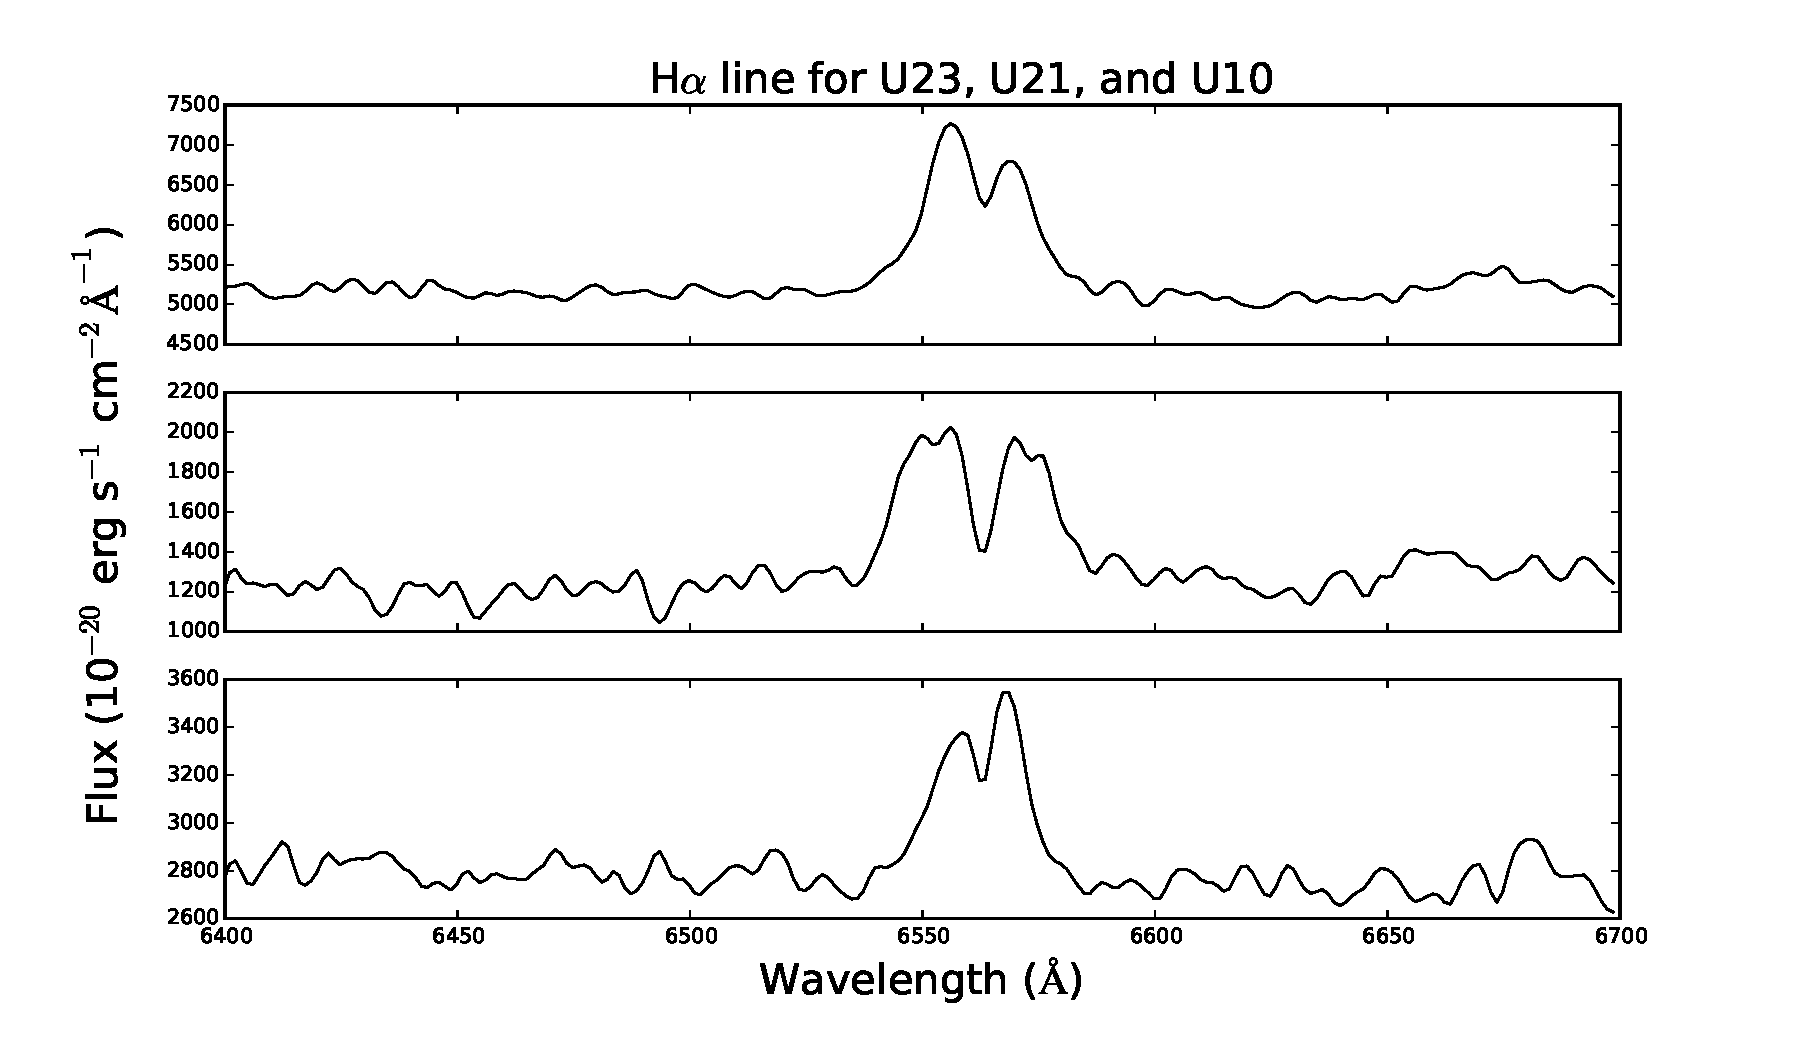
\includegraphics[scale=.5]{assets/images/todos.pdf}
\caption{Zoom of the spectra around H$\alpha$ for U23 (top), U21 (middle), and U10 (bottom)}
\label{fig:halphatodos}
\end{figure}

\begin{figure}[]
        \centering
        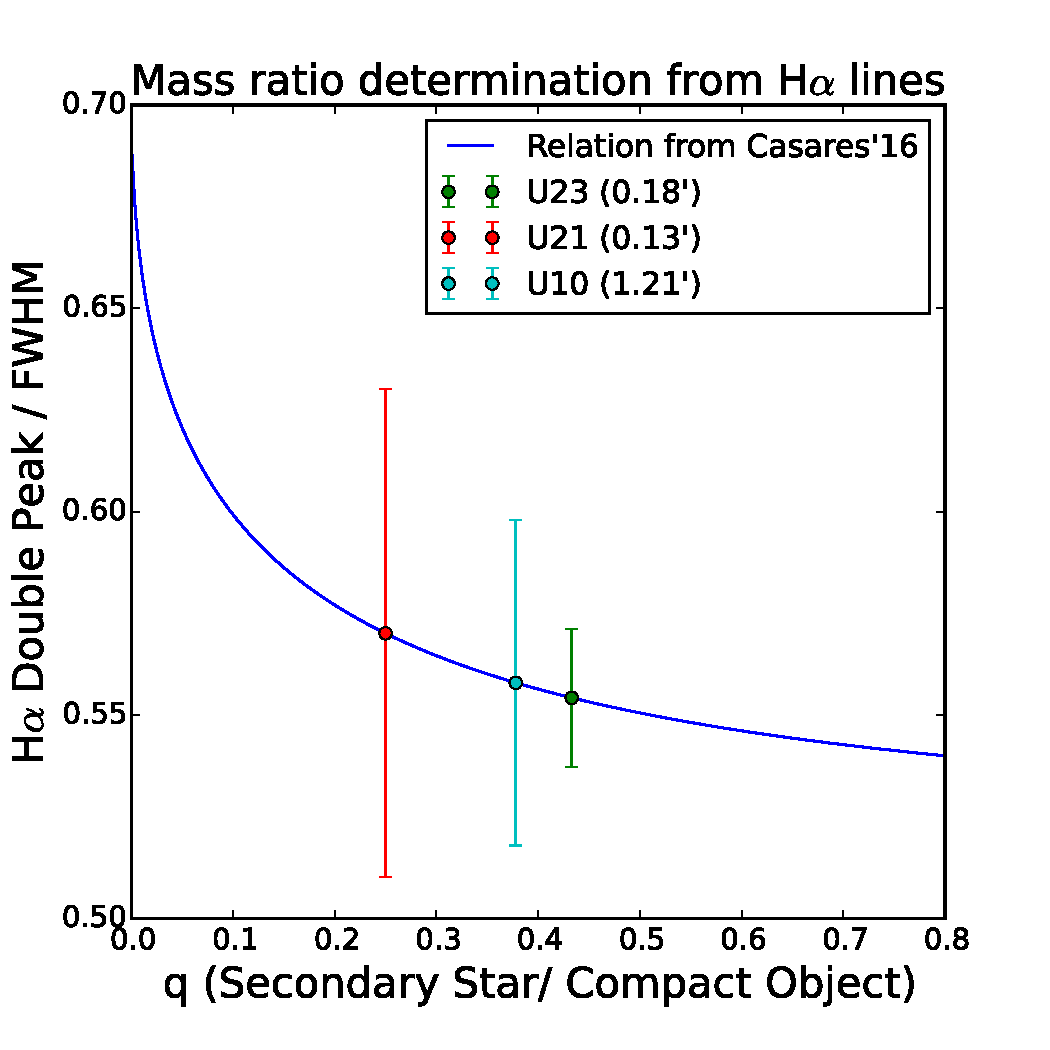
\includegraphics[scale=.5]{assets/images/mass.pdf}
\caption{The solid line is the relation between the ratio of H$\alpha$ double peak separation to Full width at half maximum (FWHM) and the mass ratio q (companion star mass over white dwarf mass) from \cite{casares_massration_20016}. Our measured values for the CVs are shown as points with their error bars. The values in parenthesis are the projected distance to the cluster center for each CV. The value of q for U23 is 0.433, for U21 is 0.25 and 0.3 for U10.}
\label{fig:mass}
\end{figure}

\subsection{Radial Velocity}

With the 8 different exposures of the center region and the strong H$\alpha$ line emission the radial velocity evolution of the CV can be traced. This is done by employing the cross-correlation algorithms of \cite{tonry_cross_1979}, as implemented in the IRAF Radial Velocity Analysis Package. This was done for U23, one of the brightest and one of the only two CVs in NGC 6397 for which the orbital period has been measured \citep{kaluzny_time_2003}. The first exposure of 25 second for the first night was used as the reference to calculate radial velocity shifts. No significant radial velocity was detected between each individual short exposure.  The same procedure to determine the radial velocity shift between the combined exposures for the first night and for the second observing night. We obtained an estimate of $23.4 \pm 14 \text{ km/s}$, which is not significant enough to claim a detected RV variation. 



%with good
%confidence (with the parameter R parameter of Tonry & Davis greater than 3).

\begin{comment}
\begin{figure}
        \centering
        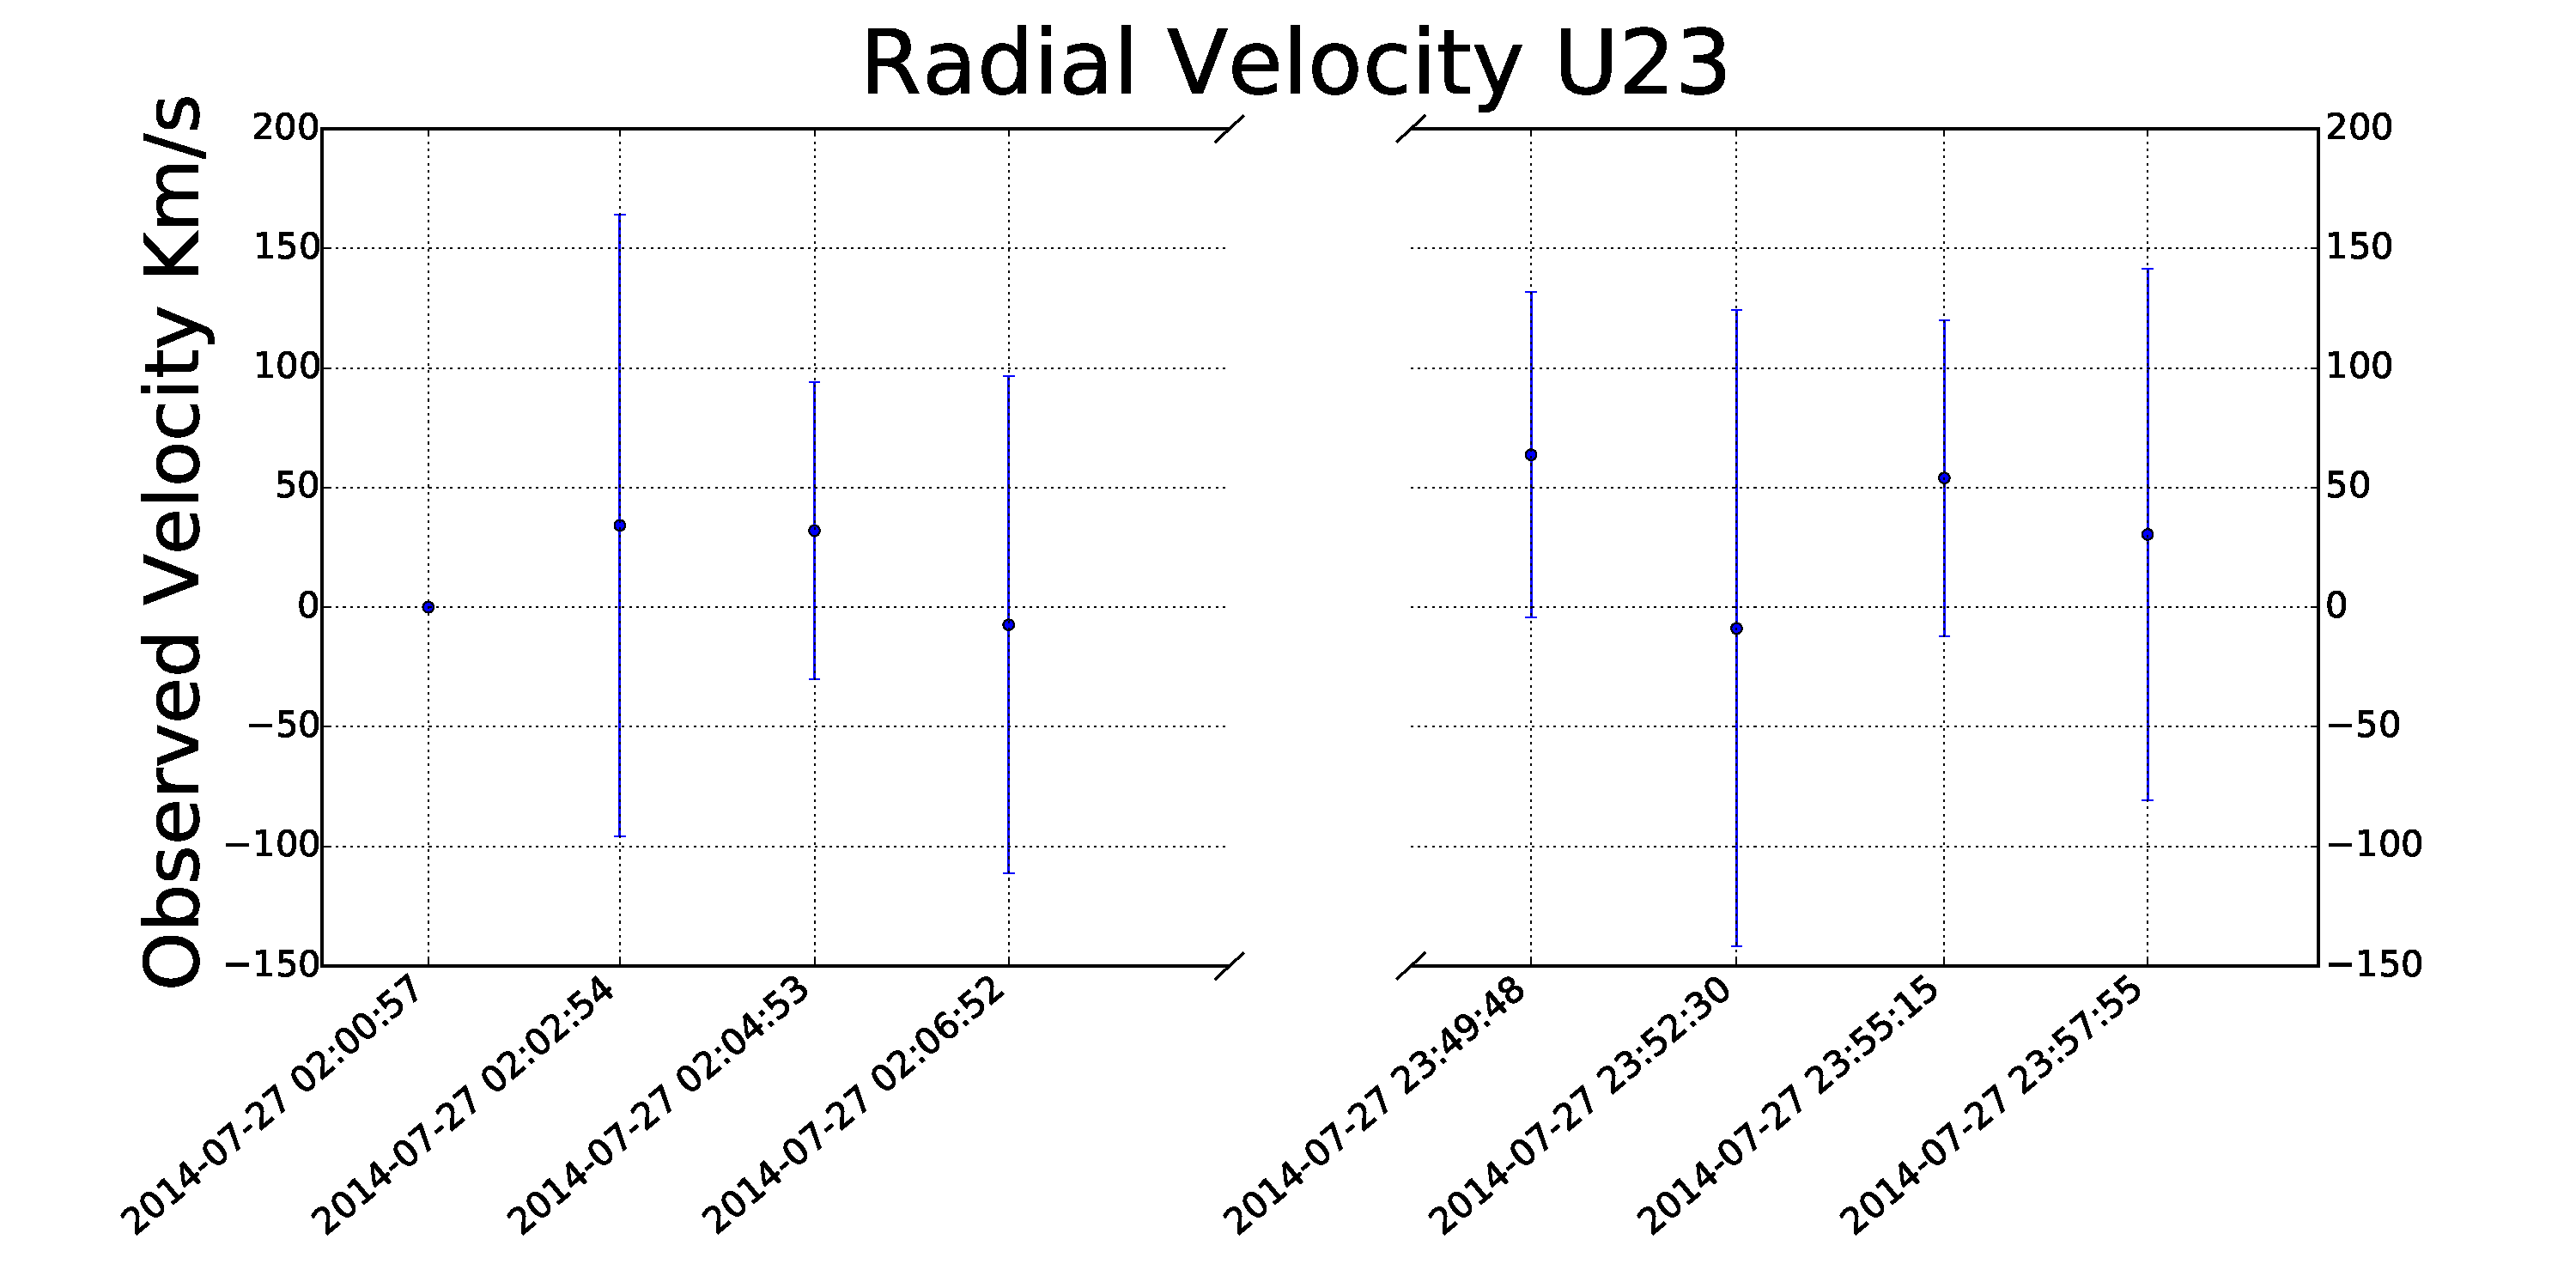
\includegraphics[scale=.3]{assets/images/radU23.pdf}
\caption{Radial velocity shift for U23. The radial velocity are measured using the first observing night as the reference template. With the available data we were unable to get a good estimate on the period of the CVs in NGC 6397, longer exposure time to obtained better quality spectra is needed.}
\label{fig:radU23}
\end{figure}
\end{comment}

%\textbf{Note for Natalie: I am not sure what velocity from fxcor. Or the error. I The }

\section{Low-mass X-ray Binary}


Besides the population of CVs in NGC 6397 we also studied a LMXB located near the center in NGC 6397. The goal was to detect possible H$\alpha$ emmision from the LMXB. The detection of hydrogen lines in the LMXB  will remove any ambiguities regarding the composition of the neutron star atmosphere. The absence of hydrogen  would be an argument for using a Helium atmosphere model resulting different mass-radius relations than for a hydrogen model. This will help better constrain the equation of state of neutron stars (see Section~\ref{sec:ns}). Using all the available observations of the center, we estimated the flux in the H $\alpha$ band to be $8.2 \times 10^{-18}$ erg/s/cm$^2$. This is a very faint object (R magnitude of $\sim 26$, \cite{heinke_improved_2014}). Longer integration time is needed to be able to obtain a spectra with a good signal-to-noise ratio and study the spectra of the LMXB. 

